% =============================================================================
% fig_security_matrix.tex  —  TikZ security property comparison matrix
% Scaled with \resizebox to strictly fit within \columnwidth in both
% two-column and single-column modes without overlapping adjacent text.
% Include with:  % =============================================================================
% fig_security_matrix.tex  —  TikZ security property comparison matrix
% Scaled with \resizebox to strictly fit within \columnwidth in both
% two-column and single-column modes without overlapping adjacent text.
% Include with:  % =============================================================================
% fig_security_matrix.tex  —  TikZ security property comparison matrix
% Scaled with \resizebox to strictly fit within \columnwidth in both
% two-column and single-column modes without overlapping adjacent text.
% Include with:  % =============================================================================
% fig_security_matrix.tex  —  TikZ security property comparison matrix
% Scaled with \resizebox to strictly fit within \columnwidth in both
% two-column and single-column modes without overlapping adjacent text.
% Include with:  \input{figures/fig_security_matrix}
% =============================================================================
\begin{figure}[!t]
\centering
\resizebox{\columnwidth}{!}{%
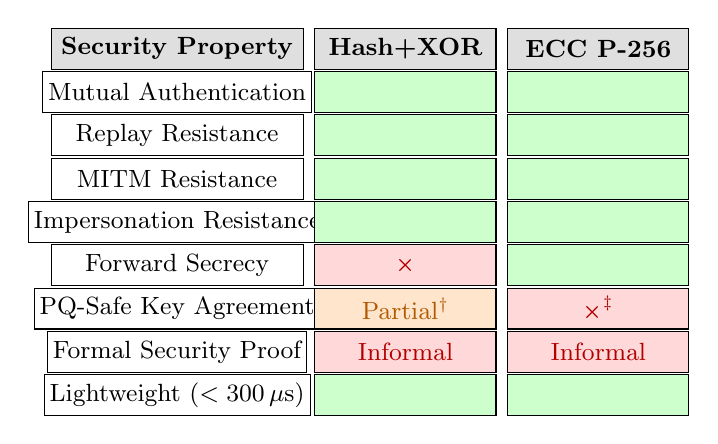
\begin{tikzpicture}[
  font=\small,
  cell/.style={draw, minimum width=2.3cm, minimum height=0.52cm,
               inner sep=2pt, align=center},
  header/.style={cell, fill=gray!25, font=\small\bfseries},
  yes/.style={cell, fill=green!20, text=green!50!black},
  no/.style={cell, fill=red!15, text=red!70!black},
  partial/.style={cell, fill=orange!20, text=orange!70!black},
]
% ---- Header row ----
\node[header, minimum width=3.2cm] (h0) at (0,0) {Security Property};
\node[header] (h1) at (2.9,0) {Hash+XOR};
\node[header] (h2) at (5.35,0) {ECC P-256};

% ---- Row 1: Mutual Authentication ----
\node[cell, minimum width=3.2cm] at (0,-0.55) {Mutual Authentication};
\node[yes]  at (2.9,-0.55) {\checkmark};
\node[yes]  at (5.35,-0.55) {\checkmark};

% ---- Row 2: Replay Resistance ----
\node[cell, minimum width=3.2cm] at (0,-1.1) {Replay Resistance};
\node[yes]  at (2.9,-1.1) {\checkmark};
\node[yes]  at (5.35,-1.1) {\checkmark};

% ---- Row 3: MITM / Tampering Resistance ----
\node[cell, minimum width=3.2cm] at (0,-1.65) {MITM Resistance};
\node[yes]  at (2.9,-1.65) {\checkmark};
\node[yes]  at (5.35,-1.65) {\checkmark};

% ---- Row 4: Impersonation Resistance ----
\node[cell, minimum width=3.2cm] at (0,-2.2) {Impersonation Resistance};
\node[yes]  at (2.9,-2.2) {\checkmark};
\node[yes]  at (5.35,-2.2) {\checkmark};

% ---- Row 5: Forward Secrecy ----
\node[cell, minimum width=3.2cm] at (0,-2.75) {Forward Secrecy};
\node[no]   at (2.9,-2.75) {\texttimes};
\node[yes]  at (5.35,-2.75) {\checkmark};

% ---- Row 6: PQ-Safe Key Agreement ----
\node[cell, minimum width=3.2cm] at (0,-3.3) {PQ-Safe Key Agreement};
\node[partial] at (2.9,-3.3) {Partial$^\dagger$};
\node[no]   at (5.35,-3.3) {\texttimes$^\ddagger$};

% ---- Row 7: Formal Security Proof ----
\node[cell, minimum width=3.2cm] at (0,-3.85) {Formal Security Proof};
\node[no]   at (2.9,-3.85) {Informal};
\node[no]   at (5.35,-3.85) {Informal};

% ---- Row 8: Lightweight (< 300 µs) ----
\node[cell, minimum width=3.2cm] at (0,-4.4) {Lightweight ($<300\,\mu$s)};
\node[yes]  at (2.9,-4.4) {\checkmark};
\node[yes]  at (5.35,-4.4) {\checkmark};

\end{tikzpicture}%
}
\vspace{4pt}

\begin{minipage}{\columnwidth}
\footnotesize
  $^\dagger$ SHA-256 security reduces to $\approx$128-bit equivalent under Grover;
  still considered adequate~\cite{NISTFIPS1804}.\\
  $^\ddagger$ ECDLP is broken in polynomial time by Shor's algorithm~\cite{Shor1997}.
  Forward secrecy holds classically but not against a quantum adversary.
\end{minipage}

\caption{Security property comparison matrix for the Hash+XOR (Ju-Park) and
ECC P-256 schemes. \checkmark = property satisfied; \texttimes = property not
satisfied; Partial = weakened but not broken. Results are based on informal
security analysis (Section~\ref{sec:security}) and primitive-level
post-quantum analysis (Section~\ref{sec:pq}).}
\label{fig:security_matrix}
\end{figure}
% =============================================================================
\begin{figure}[!t]
\centering
\resizebox{\columnwidth}{!}{%
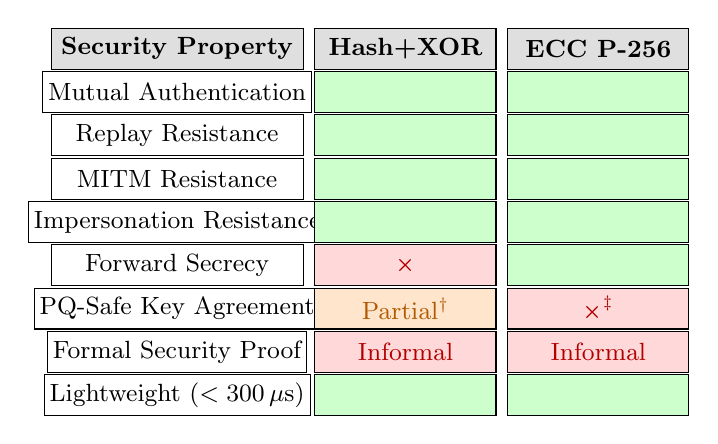
\begin{tikzpicture}[
  font=\small,
  cell/.style={draw, minimum width=2.3cm, minimum height=0.52cm,
               inner sep=2pt, align=center},
  header/.style={cell, fill=gray!25, font=\small\bfseries},
  yes/.style={cell, fill=green!20, text=green!50!black},
  no/.style={cell, fill=red!15, text=red!70!black},
  partial/.style={cell, fill=orange!20, text=orange!70!black},
]
% ---- Header row ----
\node[header, minimum width=3.2cm] (h0) at (0,0) {Security Property};
\node[header] (h1) at (2.9,0) {Hash+XOR};
\node[header] (h2) at (5.35,0) {ECC P-256};

% ---- Row 1: Mutual Authentication ----
\node[cell, minimum width=3.2cm] at (0,-0.55) {Mutual Authentication};
\node[yes]  at (2.9,-0.55) {\checkmark};
\node[yes]  at (5.35,-0.55) {\checkmark};

% ---- Row 2: Replay Resistance ----
\node[cell, minimum width=3.2cm] at (0,-1.1) {Replay Resistance};
\node[yes]  at (2.9,-1.1) {\checkmark};
\node[yes]  at (5.35,-1.1) {\checkmark};

% ---- Row 3: MITM / Tampering Resistance ----
\node[cell, minimum width=3.2cm] at (0,-1.65) {MITM Resistance};
\node[yes]  at (2.9,-1.65) {\checkmark};
\node[yes]  at (5.35,-1.65) {\checkmark};

% ---- Row 4: Impersonation Resistance ----
\node[cell, minimum width=3.2cm] at (0,-2.2) {Impersonation Resistance};
\node[yes]  at (2.9,-2.2) {\checkmark};
\node[yes]  at (5.35,-2.2) {\checkmark};

% ---- Row 5: Forward Secrecy ----
\node[cell, minimum width=3.2cm] at (0,-2.75) {Forward Secrecy};
\node[no]   at (2.9,-2.75) {\texttimes};
\node[yes]  at (5.35,-2.75) {\checkmark};

% ---- Row 6: PQ-Safe Key Agreement ----
\node[cell, minimum width=3.2cm] at (0,-3.3) {PQ-Safe Key Agreement};
\node[partial] at (2.9,-3.3) {Partial$^\dagger$};
\node[no]   at (5.35,-3.3) {\texttimes$^\ddagger$};

% ---- Row 7: Formal Security Proof ----
\node[cell, minimum width=3.2cm] at (0,-3.85) {Formal Security Proof};
\node[no]   at (2.9,-3.85) {Informal};
\node[no]   at (5.35,-3.85) {Informal};

% ---- Row 8: Lightweight (< 300 µs) ----
\node[cell, minimum width=3.2cm] at (0,-4.4) {Lightweight ($<300\,\mu$s)};
\node[yes]  at (2.9,-4.4) {\checkmark};
\node[yes]  at (5.35,-4.4) {\checkmark};

\end{tikzpicture}%
}
\vspace{4pt}

\begin{minipage}{\columnwidth}
\footnotesize
  $^\dagger$ SHA-256 security reduces to $\approx$128-bit equivalent under Grover;
  still considered adequate~\cite{NISTFIPS1804}.\\
  $^\ddagger$ ECDLP is broken in polynomial time by Shor's algorithm~\cite{Shor1997}.
  Forward secrecy holds classically but not against a quantum adversary.
\end{minipage}

\caption{Security property comparison matrix for the Hash+XOR (Ju-Park) and
ECC P-256 schemes. \checkmark = property satisfied; \texttimes = property not
satisfied; Partial = weakened but not broken. Results are based on informal
security analysis (Section~\ref{sec:security}) and primitive-level
post-quantum analysis (Section~\ref{sec:pq}).}
\label{fig:security_matrix}
\end{figure}
% =============================================================================
\begin{figure}[!t]
\centering
\resizebox{\columnwidth}{!}{%
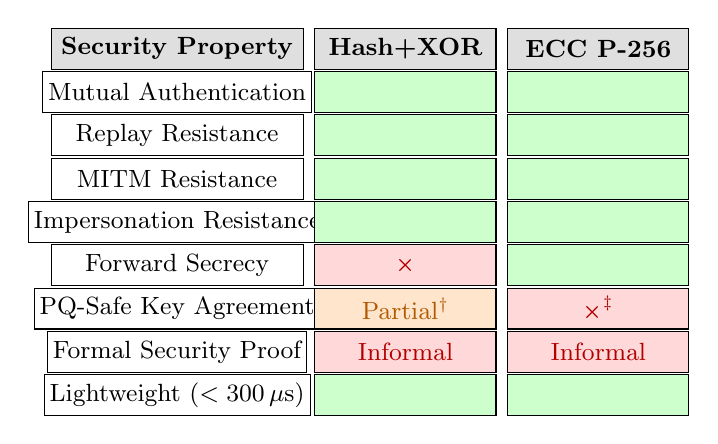
\begin{tikzpicture}[
  font=\small,
  cell/.style={draw, minimum width=2.3cm, minimum height=0.52cm,
               inner sep=2pt, align=center},
  header/.style={cell, fill=gray!25, font=\small\bfseries},
  yes/.style={cell, fill=green!20, text=green!50!black},
  no/.style={cell, fill=red!15, text=red!70!black},
  partial/.style={cell, fill=orange!20, text=orange!70!black},
]
% ---- Header row ----
\node[header, minimum width=3.2cm] (h0) at (0,0) {Security Property};
\node[header] (h1) at (2.9,0) {Hash+XOR};
\node[header] (h2) at (5.35,0) {ECC P-256};

% ---- Row 1: Mutual Authentication ----
\node[cell, minimum width=3.2cm] at (0,-0.55) {Mutual Authentication};
\node[yes]  at (2.9,-0.55) {\checkmark};
\node[yes]  at (5.35,-0.55) {\checkmark};

% ---- Row 2: Replay Resistance ----
\node[cell, minimum width=3.2cm] at (0,-1.1) {Replay Resistance};
\node[yes]  at (2.9,-1.1) {\checkmark};
\node[yes]  at (5.35,-1.1) {\checkmark};

% ---- Row 3: MITM / Tampering Resistance ----
\node[cell, minimum width=3.2cm] at (0,-1.65) {MITM Resistance};
\node[yes]  at (2.9,-1.65) {\checkmark};
\node[yes]  at (5.35,-1.65) {\checkmark};

% ---- Row 4: Impersonation Resistance ----
\node[cell, minimum width=3.2cm] at (0,-2.2) {Impersonation Resistance};
\node[yes]  at (2.9,-2.2) {\checkmark};
\node[yes]  at (5.35,-2.2) {\checkmark};

% ---- Row 5: Forward Secrecy ----
\node[cell, minimum width=3.2cm] at (0,-2.75) {Forward Secrecy};
\node[no]   at (2.9,-2.75) {\texttimes};
\node[yes]  at (5.35,-2.75) {\checkmark};

% ---- Row 6: PQ-Safe Key Agreement ----
\node[cell, minimum width=3.2cm] at (0,-3.3) {PQ-Safe Key Agreement};
\node[partial] at (2.9,-3.3) {Partial$^\dagger$};
\node[no]   at (5.35,-3.3) {\texttimes$^\ddagger$};

% ---- Row 7: Formal Security Proof ----
\node[cell, minimum width=3.2cm] at (0,-3.85) {Formal Security Proof};
\node[no]   at (2.9,-3.85) {Informal};
\node[no]   at (5.35,-3.85) {Informal};

% ---- Row 8: Lightweight (< 300 µs) ----
\node[cell, minimum width=3.2cm] at (0,-4.4) {Lightweight ($<300\,\mu$s)};
\node[yes]  at (2.9,-4.4) {\checkmark};
\node[yes]  at (5.35,-4.4) {\checkmark};

\end{tikzpicture}%
}
\vspace{4pt}

\begin{minipage}{\columnwidth}
\footnotesize
  $^\dagger$ SHA-256 security reduces to $\approx$128-bit equivalent under Grover;
  still considered adequate~\cite{NISTFIPS1804}.\\
  $^\ddagger$ ECDLP is broken in polynomial time by Shor's algorithm~\cite{Shor1997}.
  Forward secrecy holds classically but not against a quantum adversary.
\end{minipage}

\caption{Security property comparison matrix for the Hash+XOR (Ju-Park) and
ECC P-256 schemes. \checkmark = property satisfied; \texttimes = property not
satisfied; Partial = weakened but not broken. Results are based on informal
security analysis (Section~\ref{sec:security}) and primitive-level
post-quantum analysis (Section~\ref{sec:pq}).}
\label{fig:security_matrix}
\end{figure}
% =============================================================================
\begin{figure}[!t]
\centering
\resizebox{\columnwidth}{!}{%
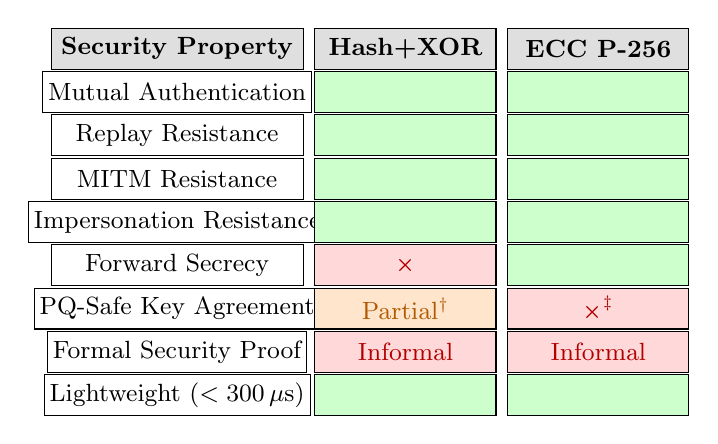
\begin{tikzpicture}[
  font=\small,
  cell/.style={draw, minimum width=2.3cm, minimum height=0.52cm,
               inner sep=2pt, align=center},
  header/.style={cell, fill=gray!25, font=\small\bfseries},
  yes/.style={cell, fill=green!20, text=green!50!black},
  no/.style={cell, fill=red!15, text=red!70!black},
  partial/.style={cell, fill=orange!20, text=orange!70!black},
]
% ---- Header row ----
\node[header, minimum width=3.2cm] (h0) at (0,0) {Security Property};
\node[header] (h1) at (2.9,0) {Hash+XOR};
\node[header] (h2) at (5.35,0) {ECC P-256};

% ---- Row 1: Mutual Authentication ----
\node[cell, minimum width=3.2cm] at (0,-0.55) {Mutual Authentication};
\node[yes]  at (2.9,-0.55) {\checkmark};
\node[yes]  at (5.35,-0.55) {\checkmark};

% ---- Row 2: Replay Resistance ----
\node[cell, minimum width=3.2cm] at (0,-1.1) {Replay Resistance};
\node[yes]  at (2.9,-1.1) {\checkmark};
\node[yes]  at (5.35,-1.1) {\checkmark};

% ---- Row 3: MITM / Tampering Resistance ----
\node[cell, minimum width=3.2cm] at (0,-1.65) {MITM Resistance};
\node[yes]  at (2.9,-1.65) {\checkmark};
\node[yes]  at (5.35,-1.65) {\checkmark};

% ---- Row 4: Impersonation Resistance ----
\node[cell, minimum width=3.2cm] at (0,-2.2) {Impersonation Resistance};
\node[yes]  at (2.9,-2.2) {\checkmark};
\node[yes]  at (5.35,-2.2) {\checkmark};

% ---- Row 5: Forward Secrecy ----
\node[cell, minimum width=3.2cm] at (0,-2.75) {Forward Secrecy};
\node[no]   at (2.9,-2.75) {\texttimes};
\node[yes]  at (5.35,-2.75) {\checkmark};

% ---- Row 6: PQ-Safe Key Agreement ----
\node[cell, minimum width=3.2cm] at (0,-3.3) {PQ-Safe Key Agreement};
\node[partial] at (2.9,-3.3) {Partial$^\dagger$};
\node[no]   at (5.35,-3.3) {\texttimes$^\ddagger$};

% ---- Row 7: Formal Security Proof ----
\node[cell, minimum width=3.2cm] at (0,-3.85) {Formal Security Proof};
\node[no]   at (2.9,-3.85) {Informal};
\node[no]   at (5.35,-3.85) {Informal};

% ---- Row 8: Lightweight (< 300 µs) ----
\node[cell, minimum width=3.2cm] at (0,-4.4) {Lightweight ($<300\,\mu$s)};
\node[yes]  at (2.9,-4.4) {\checkmark};
\node[yes]  at (5.35,-4.4) {\checkmark};

\end{tikzpicture}%
}
\vspace{4pt}

\begin{minipage}{\columnwidth}
\footnotesize
  $^\dagger$ SHA-256 security reduces to $\approx$128-bit equivalent under Grover;
  still considered adequate~\cite{NISTFIPS1804}.\\
  $^\ddagger$ ECDLP is broken in polynomial time by Shor's algorithm~\cite{Shor1997}.
  Forward secrecy holds classically but not against a quantum adversary.
\end{minipage}

\caption{Security property comparison matrix for the Hash+XOR (Ju-Park) and
ECC P-256 schemes. \checkmark = property satisfied; \texttimes = property not
satisfied; Partial = weakened but not broken. Results are based on informal
security analysis (Section~\ref{sec:security}) and primitive-level
post-quantum analysis (Section~\ref{sec:pq}).}
\label{fig:security_matrix}
\end{figure}